\section{Experimental work/analytical investigation/ design}

\subsection{采集数据}
要进行深度学习,所需要的第一步就是采集数据。在本实验中,我们使用了预先从生物实验室制备好的石蜡包埋好的组织切片(鱼的卵巢组织),将其放在HM355s自动切片机上依据切片机的使用手册,以不同的切削角度执行切片操作。记录切削数据。

%在这不要提三个点的鱼的肺泡组织,在后面作为模型二次验证和增强使用。

其中切片机(\autoref{fig:machine})的切片示意图(以牙齿为例) 如\autoref{fig:cutting_machine}所示

\begin{figure}[htbp]
    \centering
    \begin{minipage}{0.48\textwidth}
        \centering
        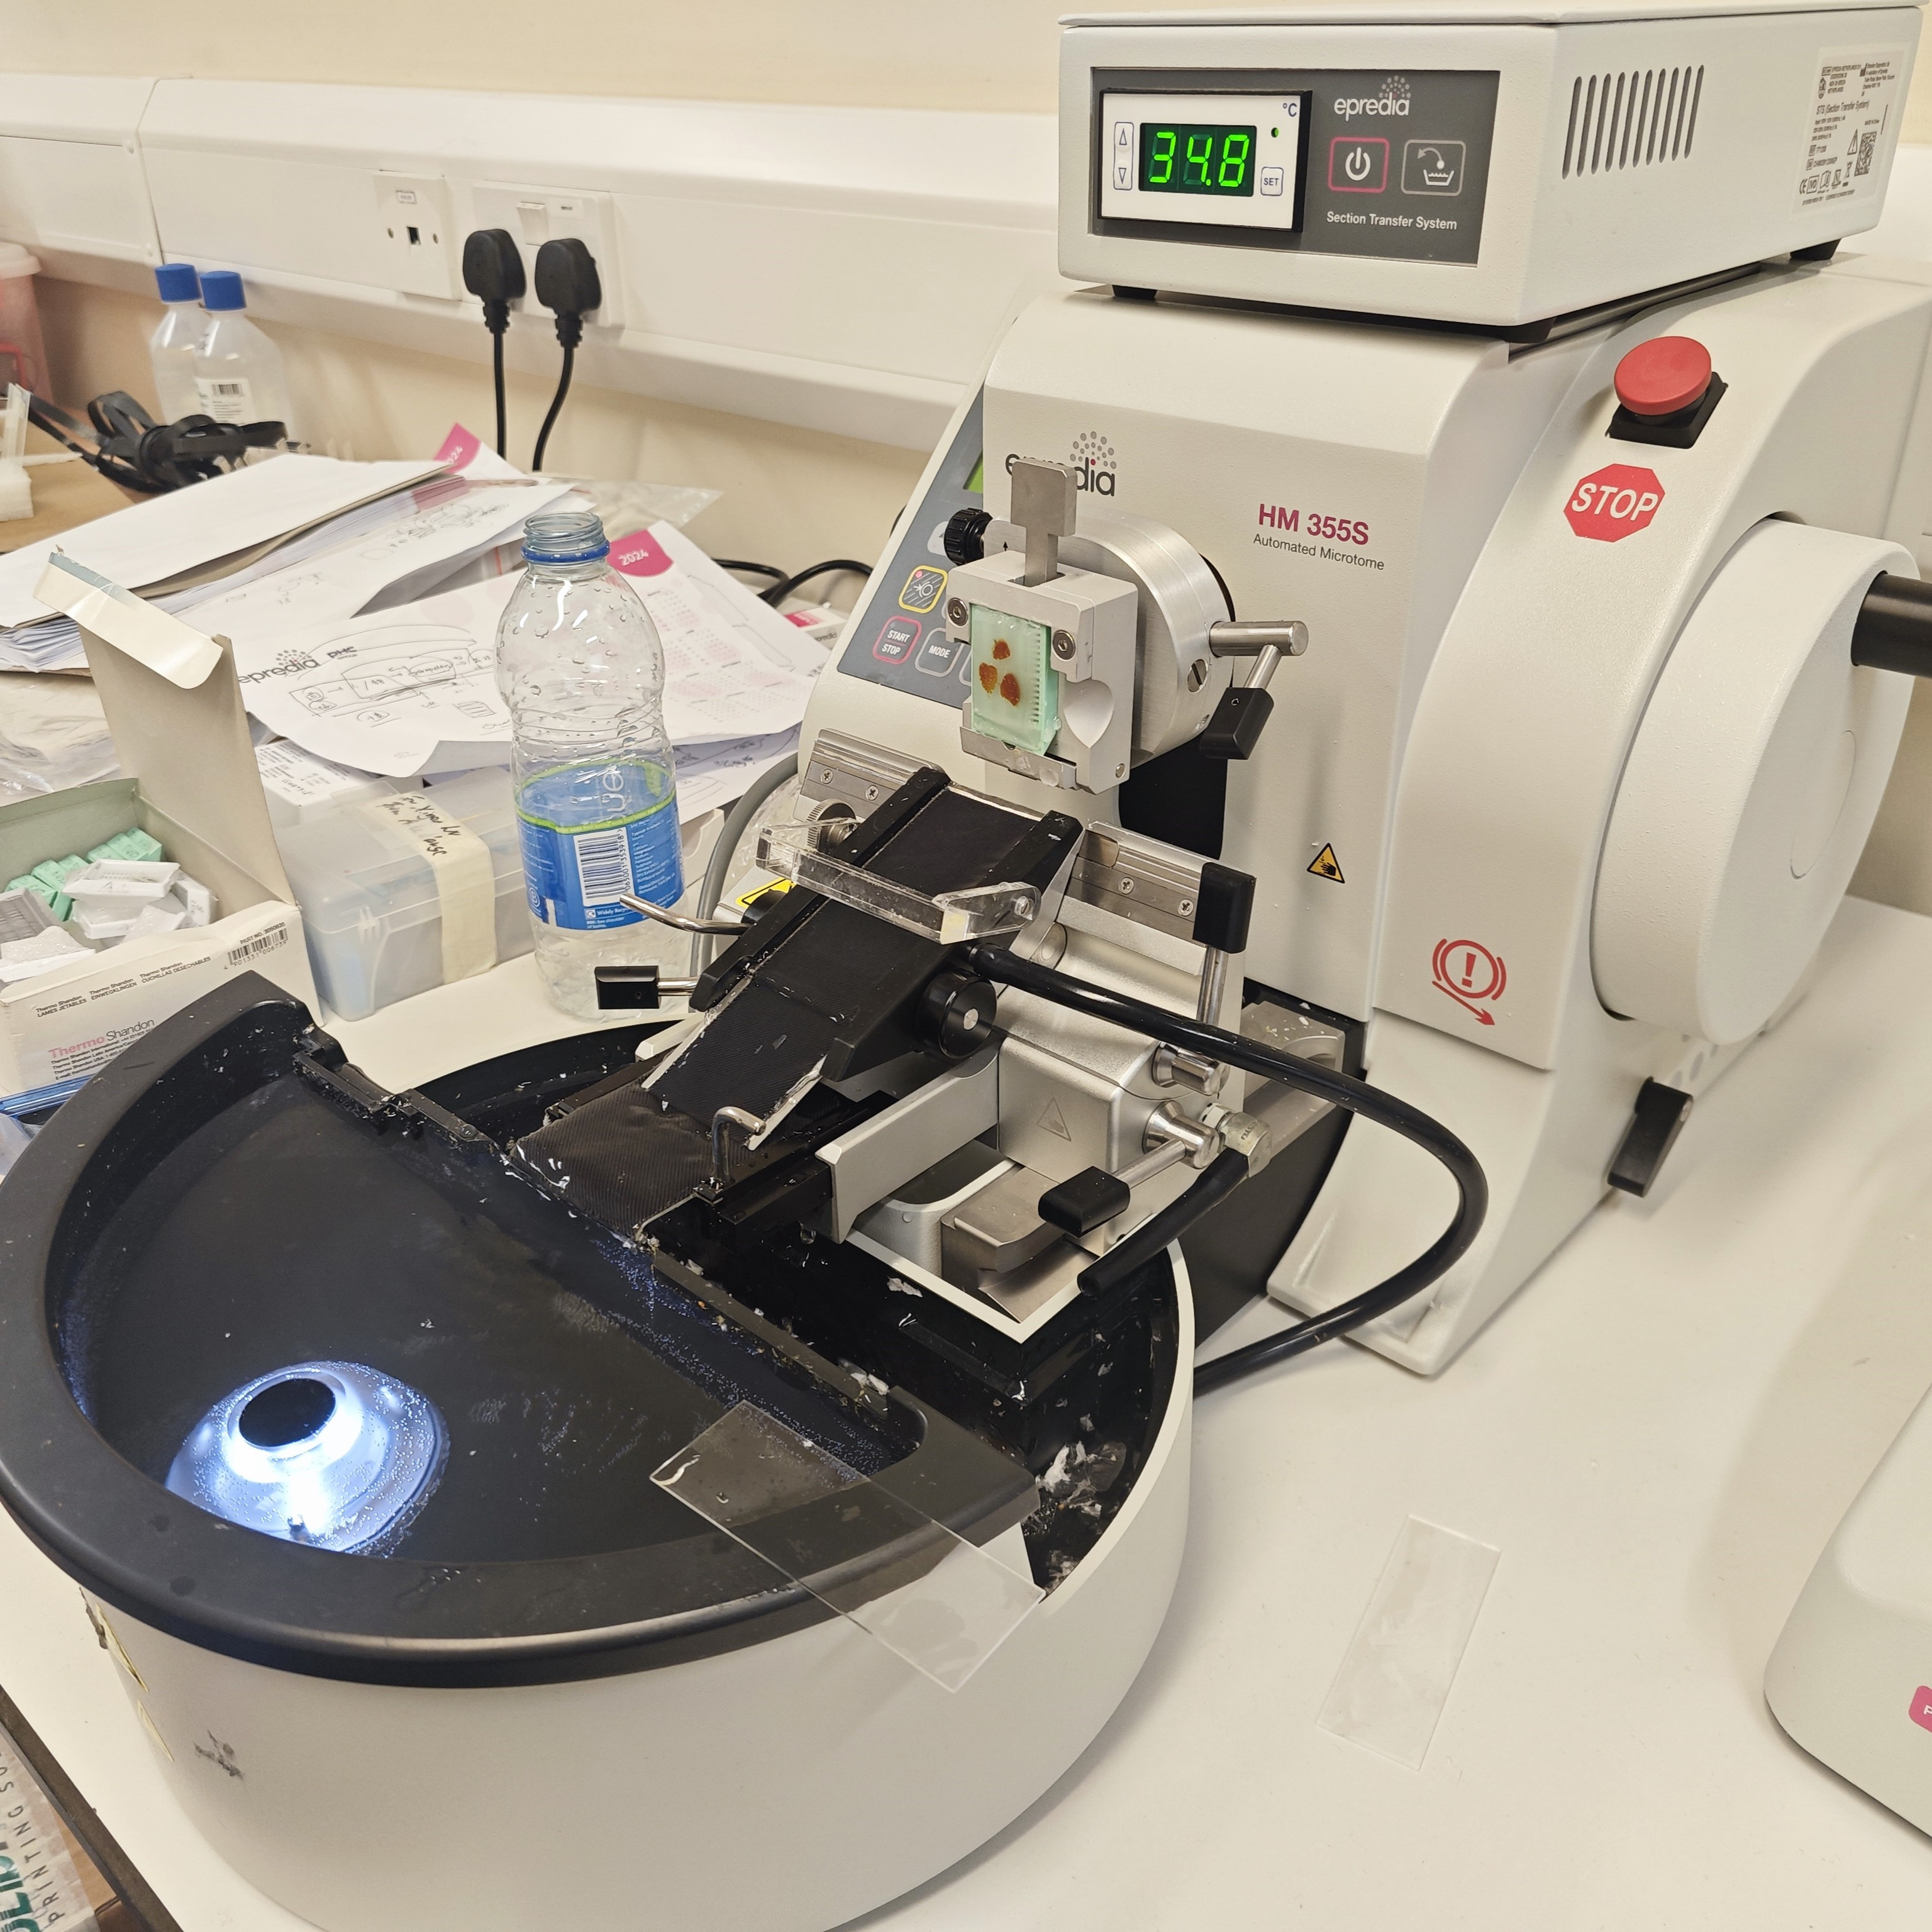
\includegraphics[width=\textwidth]{./fig/machine.jpg}
        \caption{切片机}
        \label{fig:machine}
    \end{minipage}
    \begin{minipage}{0.48\textwidth}
        \centering
        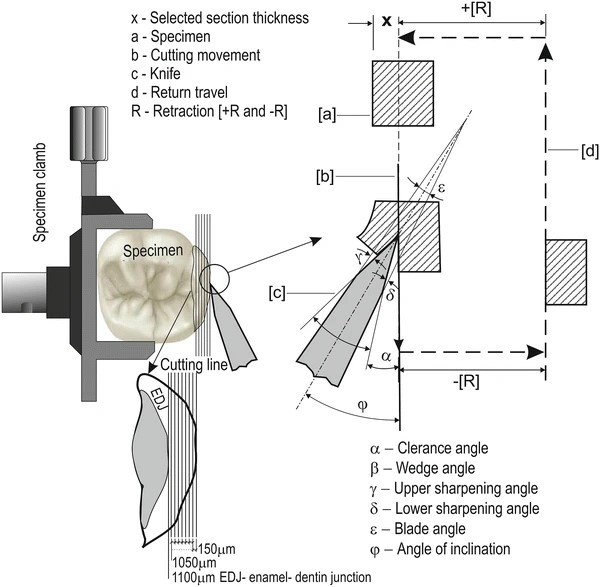
\includegraphics[width=\textwidth]{./fig/10266_2018_353_Fig1_HTML.jpg}
        \caption{切片机示意图}
        \label{fig:cutting_machine}
    \end{minipage}
\end{figure}
% https://link.springer.com/article/10.1007/s10266-018-0353-6


用于切片的生物组织(示例)如\autoref{label:sample}所示

在切削过程中,从切角为8度开始(如\autoref{fig:machine}中的angle of inclination),每次增加0.5度,直到切角为12度。切片机在切片过程中保持给进速度为25,厚度为1。

在切片完成之后,将切好的不同类型的组织切片放在载玻片上(如\autoref{fig:采集样本})所示,待其晾干后转移至VHX7000显微镜下,通过显微镜对每份样品进行拍照,获取到每份样品的电子图像数据(如\autoref{fig:显微镜})。

\begin{figure}[htbp]
    \centering
    \begin{minipage}{0.3\textwidth}
        \centering
        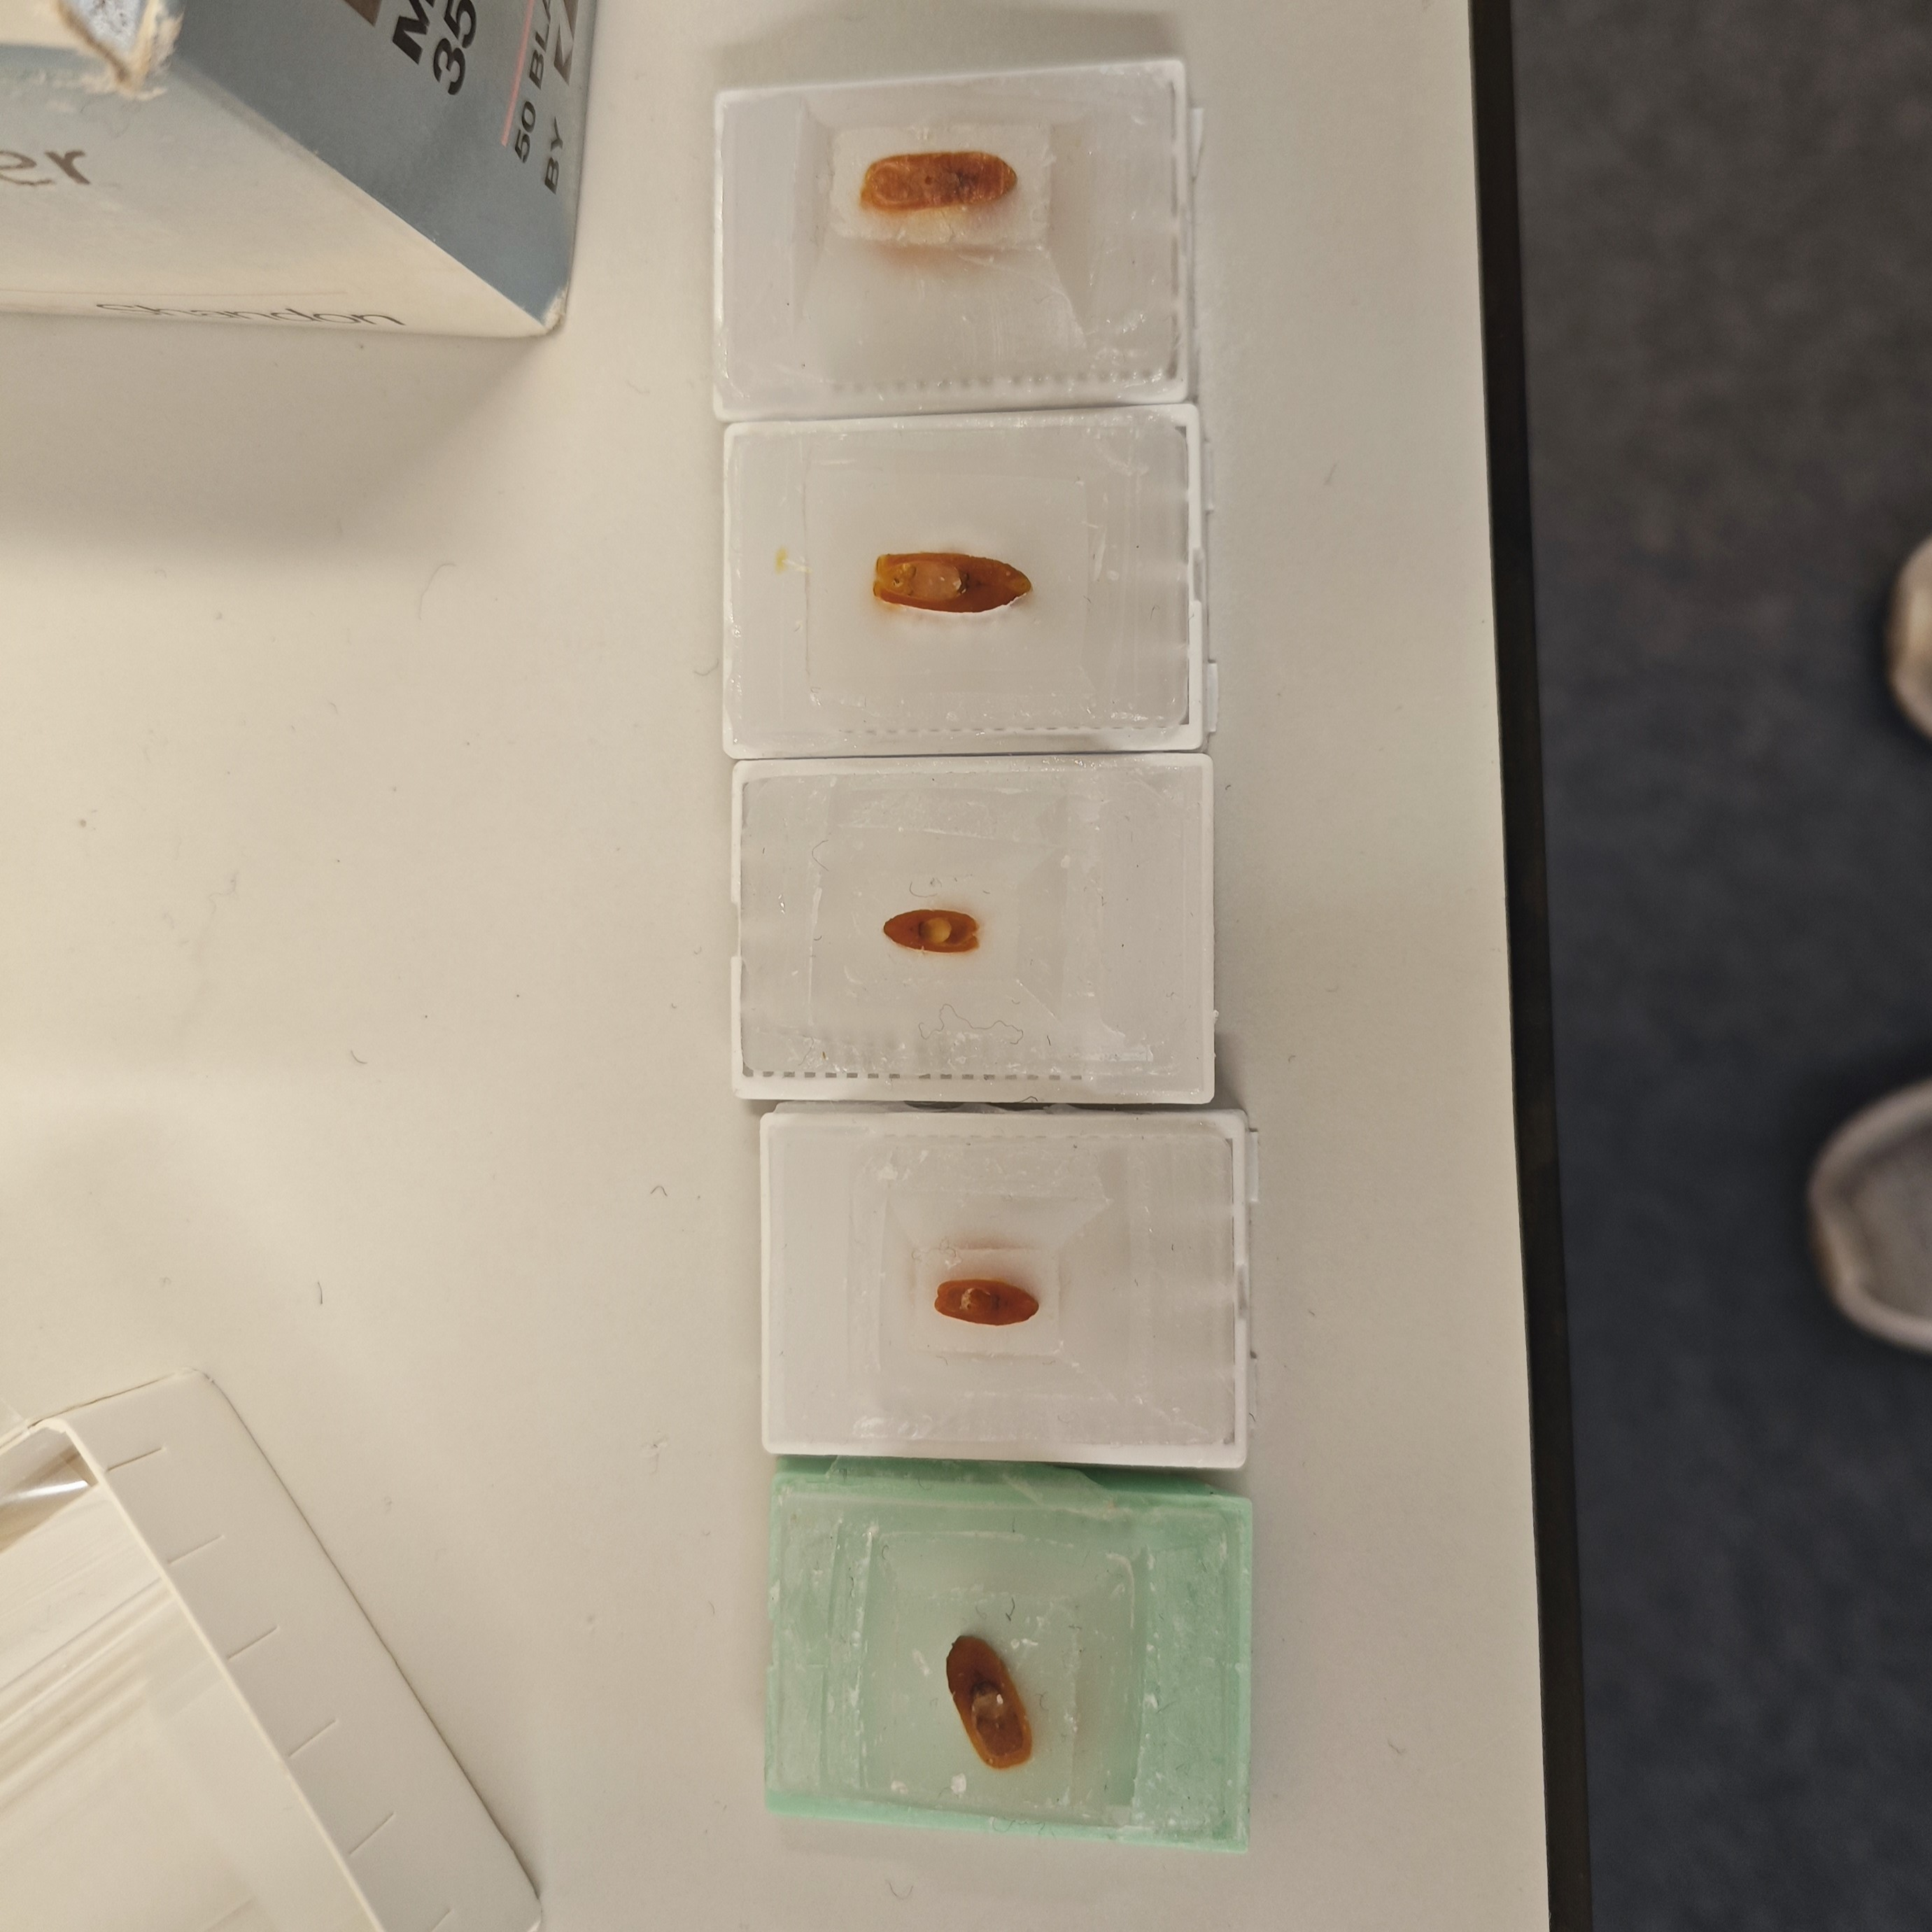
\includegraphics[width=\textwidth]{./fig/sample.jpg}
        \caption{生物组织切片}
        \label{label:sample}
    \end{minipage}
    \begin{minipage}{0.3\textwidth}
        \centering
        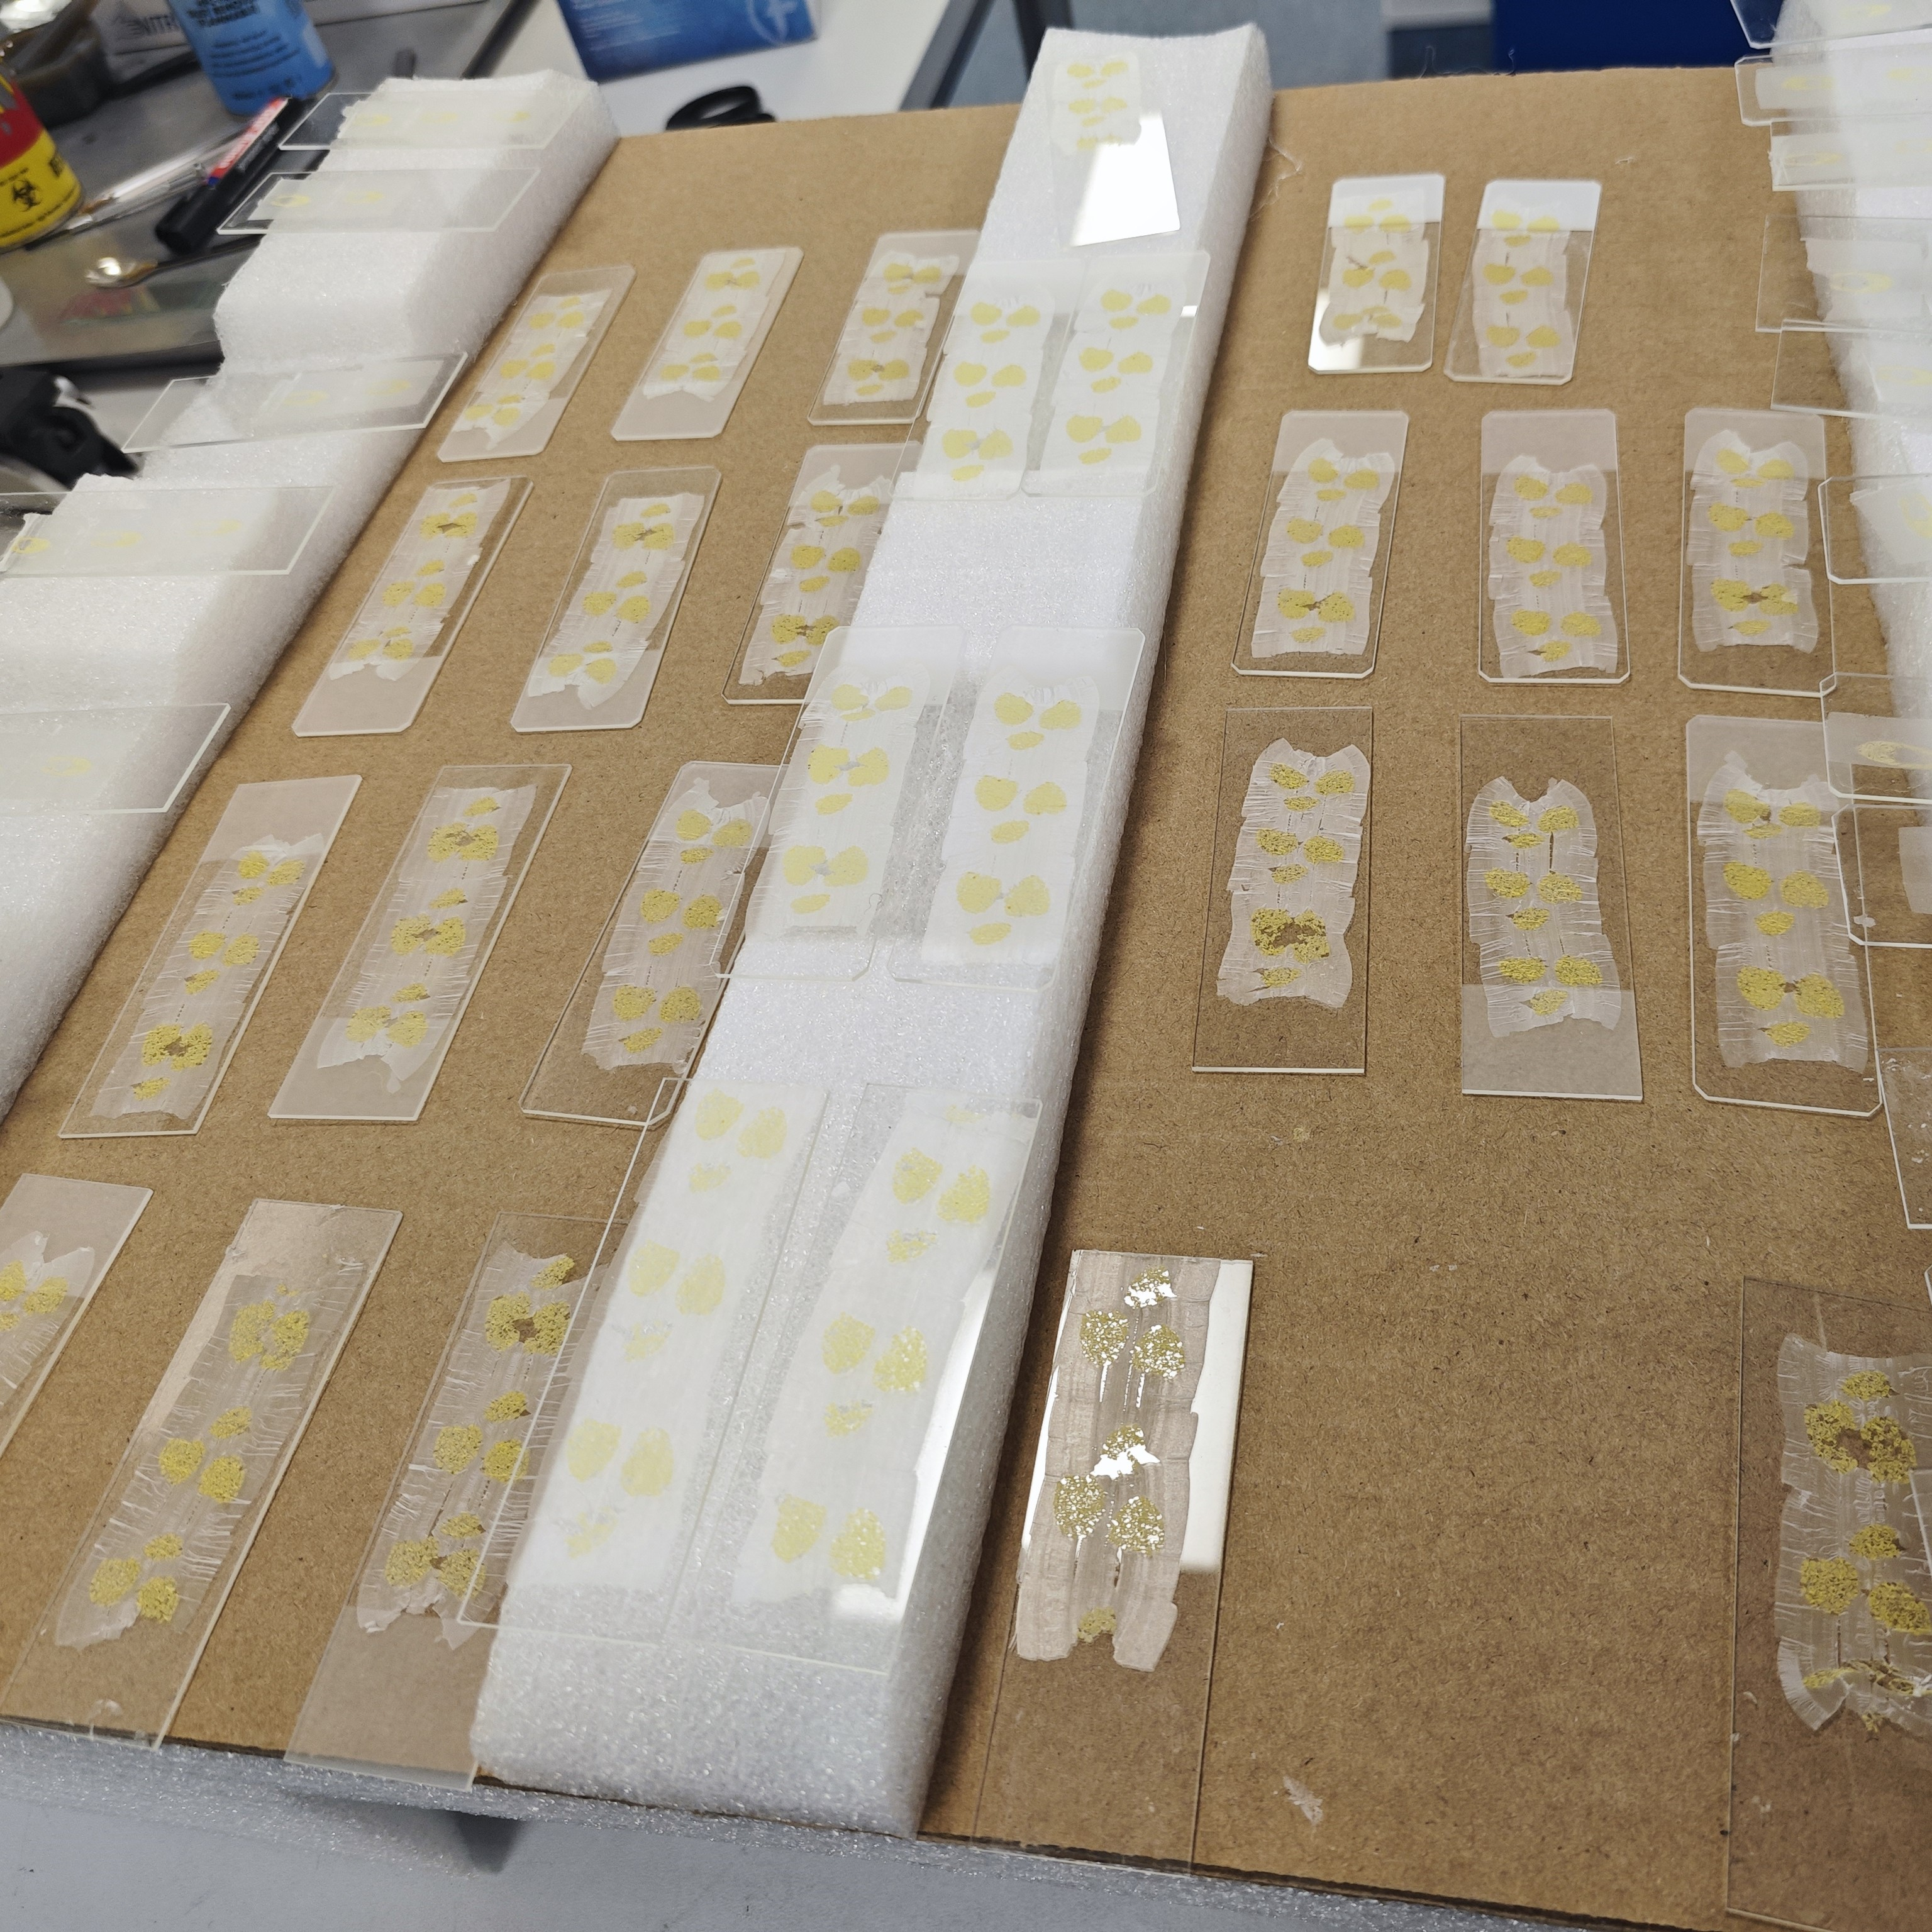
\includegraphics[width=\textwidth]{./fig/采集样本.jpg}
        \caption{采集样本}
        \label{fig:采集样本}
    \end{minipage}
    \begin{minipage}{0.35\textwidth}
        \centering
        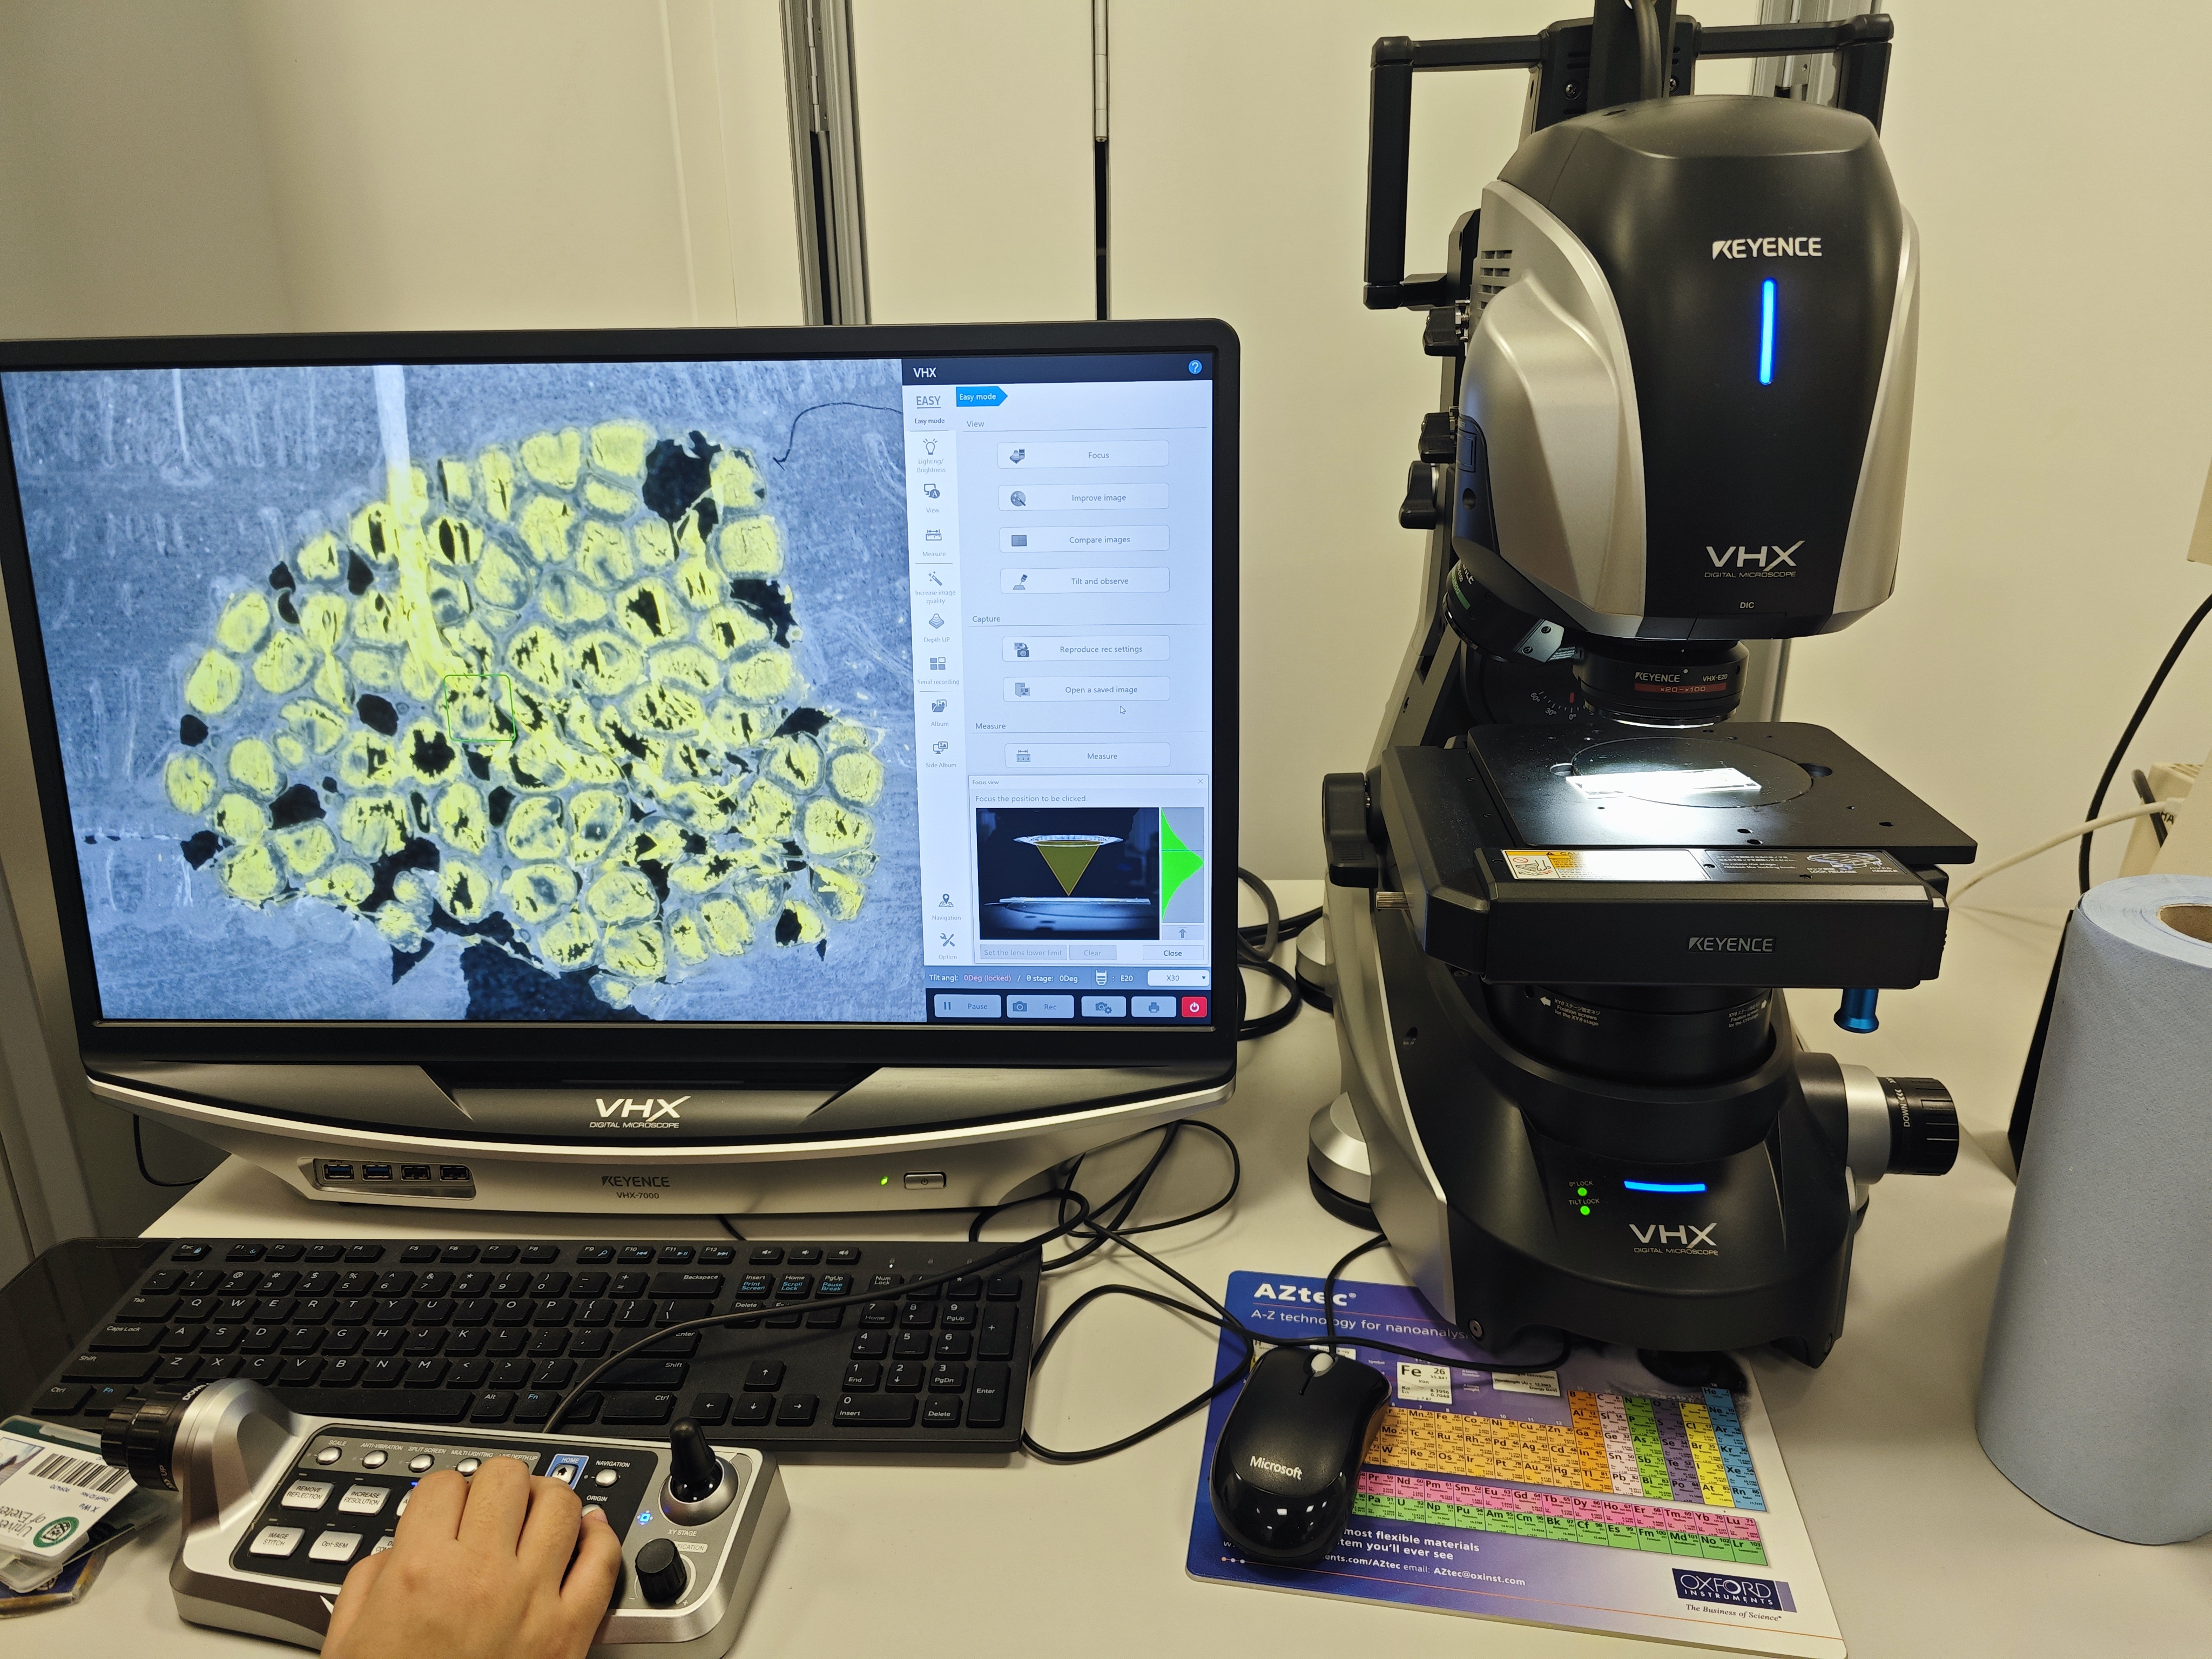
\includegraphics[width=\textwidth]{./fig/显微镜.jpg}
        \caption{显微镜}
        \label{fig:显微镜}
    \end{minipage}
\end{figure}

%图片需要后续更改为卵巢的

据此,一共得到9组数据,代表了从8到12每0.5度切角的数据。一共得到约为200张图片,每张图片的分辨率为2880*2160。其中一张(切角9.5度)如\autoref{fig:sample9.5}所示。

\begin{figure}
    \centering
    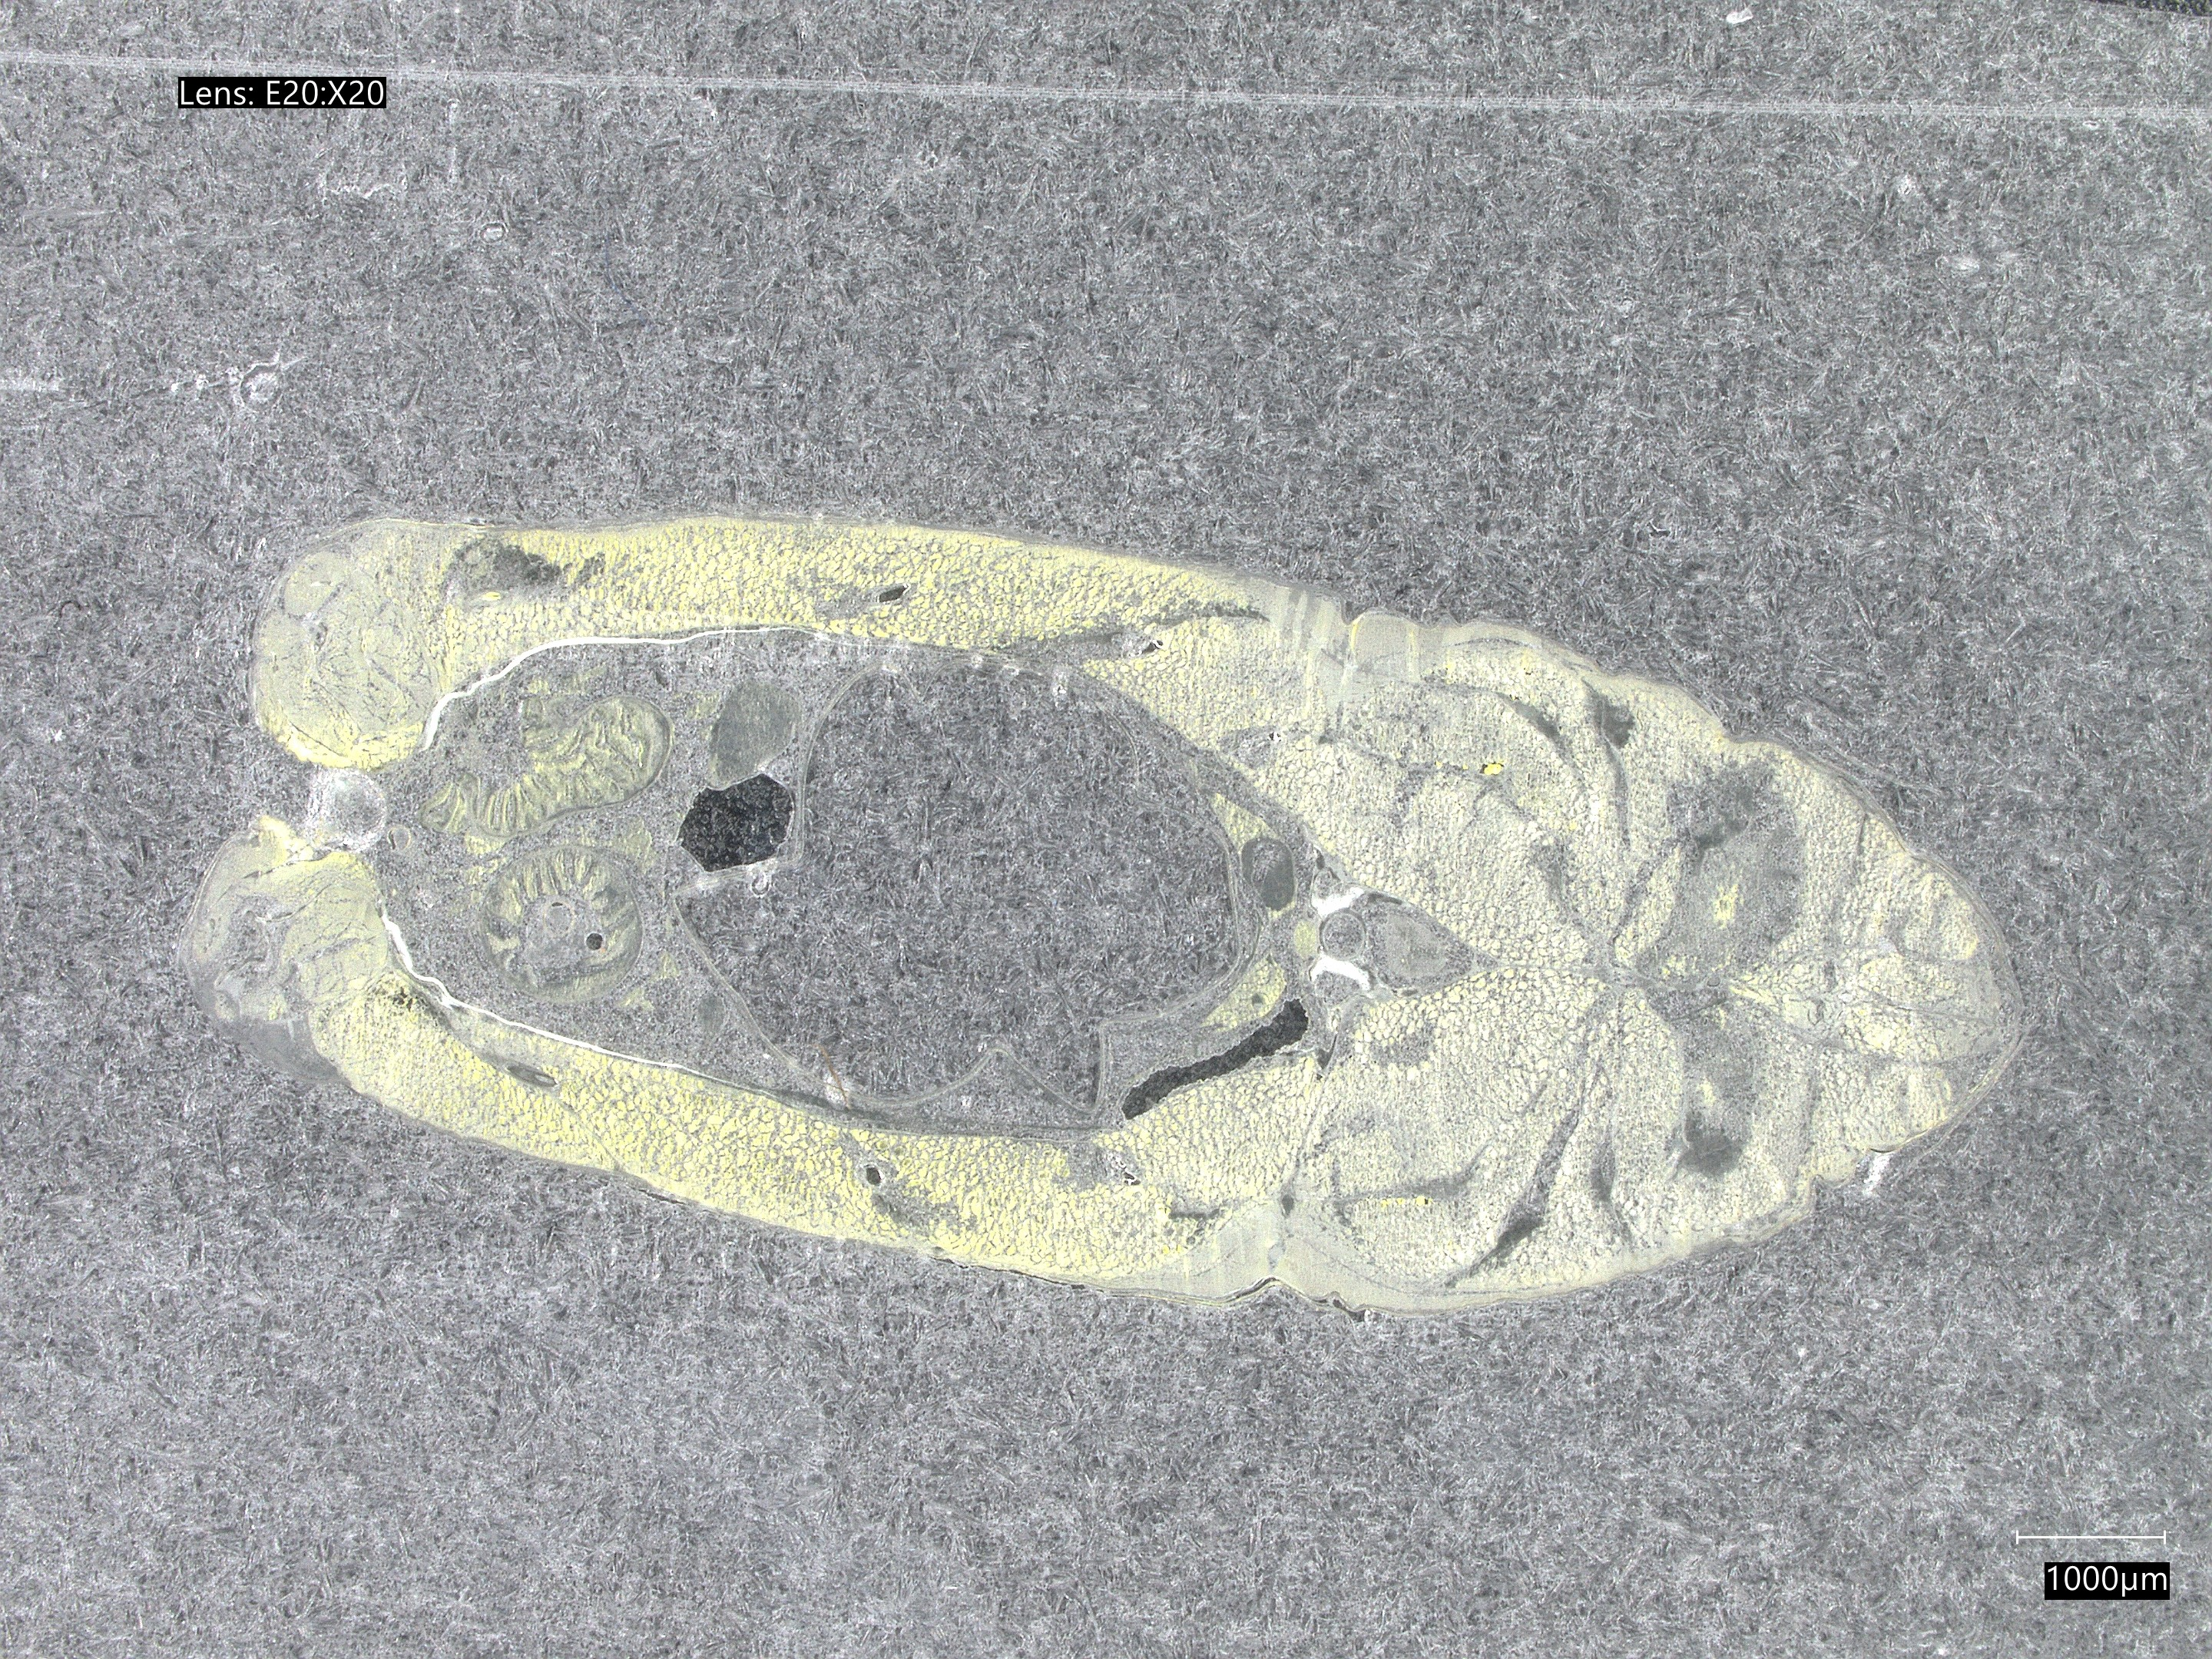
\includegraphics[width=0.8\textwidth]{./fig/sample9.5.jpg}
    \caption{切角9.5度的样本}
    \label{fig:sample9.5}
\end{figure}


这将作为我们的数据集,用于训练模型。

\subsection{模型1:原始图像+简单的cnn网络}

对于一个全新的数据集,在不确定图像复杂度对应的何种模型之前,
首先尝试一个简单的cnn网络(架构如下),以了解数据集的特点和图像复杂度。

\begin{table}
\centering
\caption{Configuration of the simple CNN model}
\begin{tabular}{ccccc}
    \toprule
    \textbf{Layer Type} & \textbf{Configuration 1} & \textbf{Configuration 2} & \textbf{Configuration 3} \\
    \midrule
    Input Layer & - & - & - \\
    Conv Layer 1 & Conv3-32 (relu) & Conv3-16 (relu) & Conv3-32 (relu) \\
    Pooling Layer 1 & MaxPooling & MaxPooling& MaxPooling \\
    Conv Layer 2 & Conv3-32 (relu) & Conv3-32 (relu) & Conv3-32 (relu) \\
    Pooling Layer 2 & MaxPooling & MaxPooling& MaxPooling \\
    Conv Layer 3 & Conv3-32 (relu) & Conv3-64 (relu) & Conv3-32 (relu) \\
    Pooling Layer 3 & MaxPooling & MaxPooling& MaxPooling \\
    Flattening Layer & Flatten() & Flatten() & Flatten() \\
    FC(Full connect) & Dense(128, relu) & Dense(128, relu) & Dense(256, relu) \\
    Output Layer & - & - & - \\
    \bottomrule
\end{tabular}

\label{tab:cnn_configuration}
\end{table}

\subsection{改进:图片预处理}

\subsection{模型2:预处理图像+简单的cnn网络}

\subsection{模型3:原始图像+迁移学习}